Although the synchronization protocol is one of the defining factors in simulation performance, model allocation has a significant impact on which protocol is ideal, and even whether or not parallelization would make sense.
Indeed, if the model is distributed in such a way that frequent communication is necessary between cores, parallelism is naturally reduced.
This thus brings us to the topic of model allocation.
Model allocation was one of the features also implemented by PythonPDEVS~\cite{PythonPDEVS2}.

The modeller can specify which kernel a model should be allocated to, should such manual intervention be required.
This is handled by the default model allocator.
If no preference is given a simple striping scheme is followed but this is not sufficient in most simulations to achieve a speedup in parallel.
By overriding the default allocator a modeller tunes the allocation scheme for a specific model, maximizing parallel speedup.
This interface can be used to employ graph algorithms for an automatic allocation scheme, for example avoiding cycles in the dependency graph.

\subsection{Performance Evaluation}
In order to evaluate the influence of model allocation, we define a new model, based on PHOLD~\cite{PHOLD}.
The model structure resembles a tree: an atomic model can have a set of children, with children being connected to each other as well.
Connections can be uni- or bidirectional.

Unlike the Queue model, the width of the hierarchy is still present in the topology of the atomic models after the direct connection stage.
The PHOLDTree model allows us to investigate parallel speedup in terms of model allocation, by modifying the depth and width (fanout) model parameters.

The PHOLDTree model is similar in structure to models of gossiping in social networks~\cite{Gossip} and multi-granularity locking~\cite{MultiGranularityLocking}.
The lookahead of an atomic node is the minimally allowed $\epsilon$, indicating uncertainty, as is often the case in realistic models.
We demonstrate the importance of allocation, by comparing a breadth-first versus a depth-first scheme.

\begin{figure}
    \center
    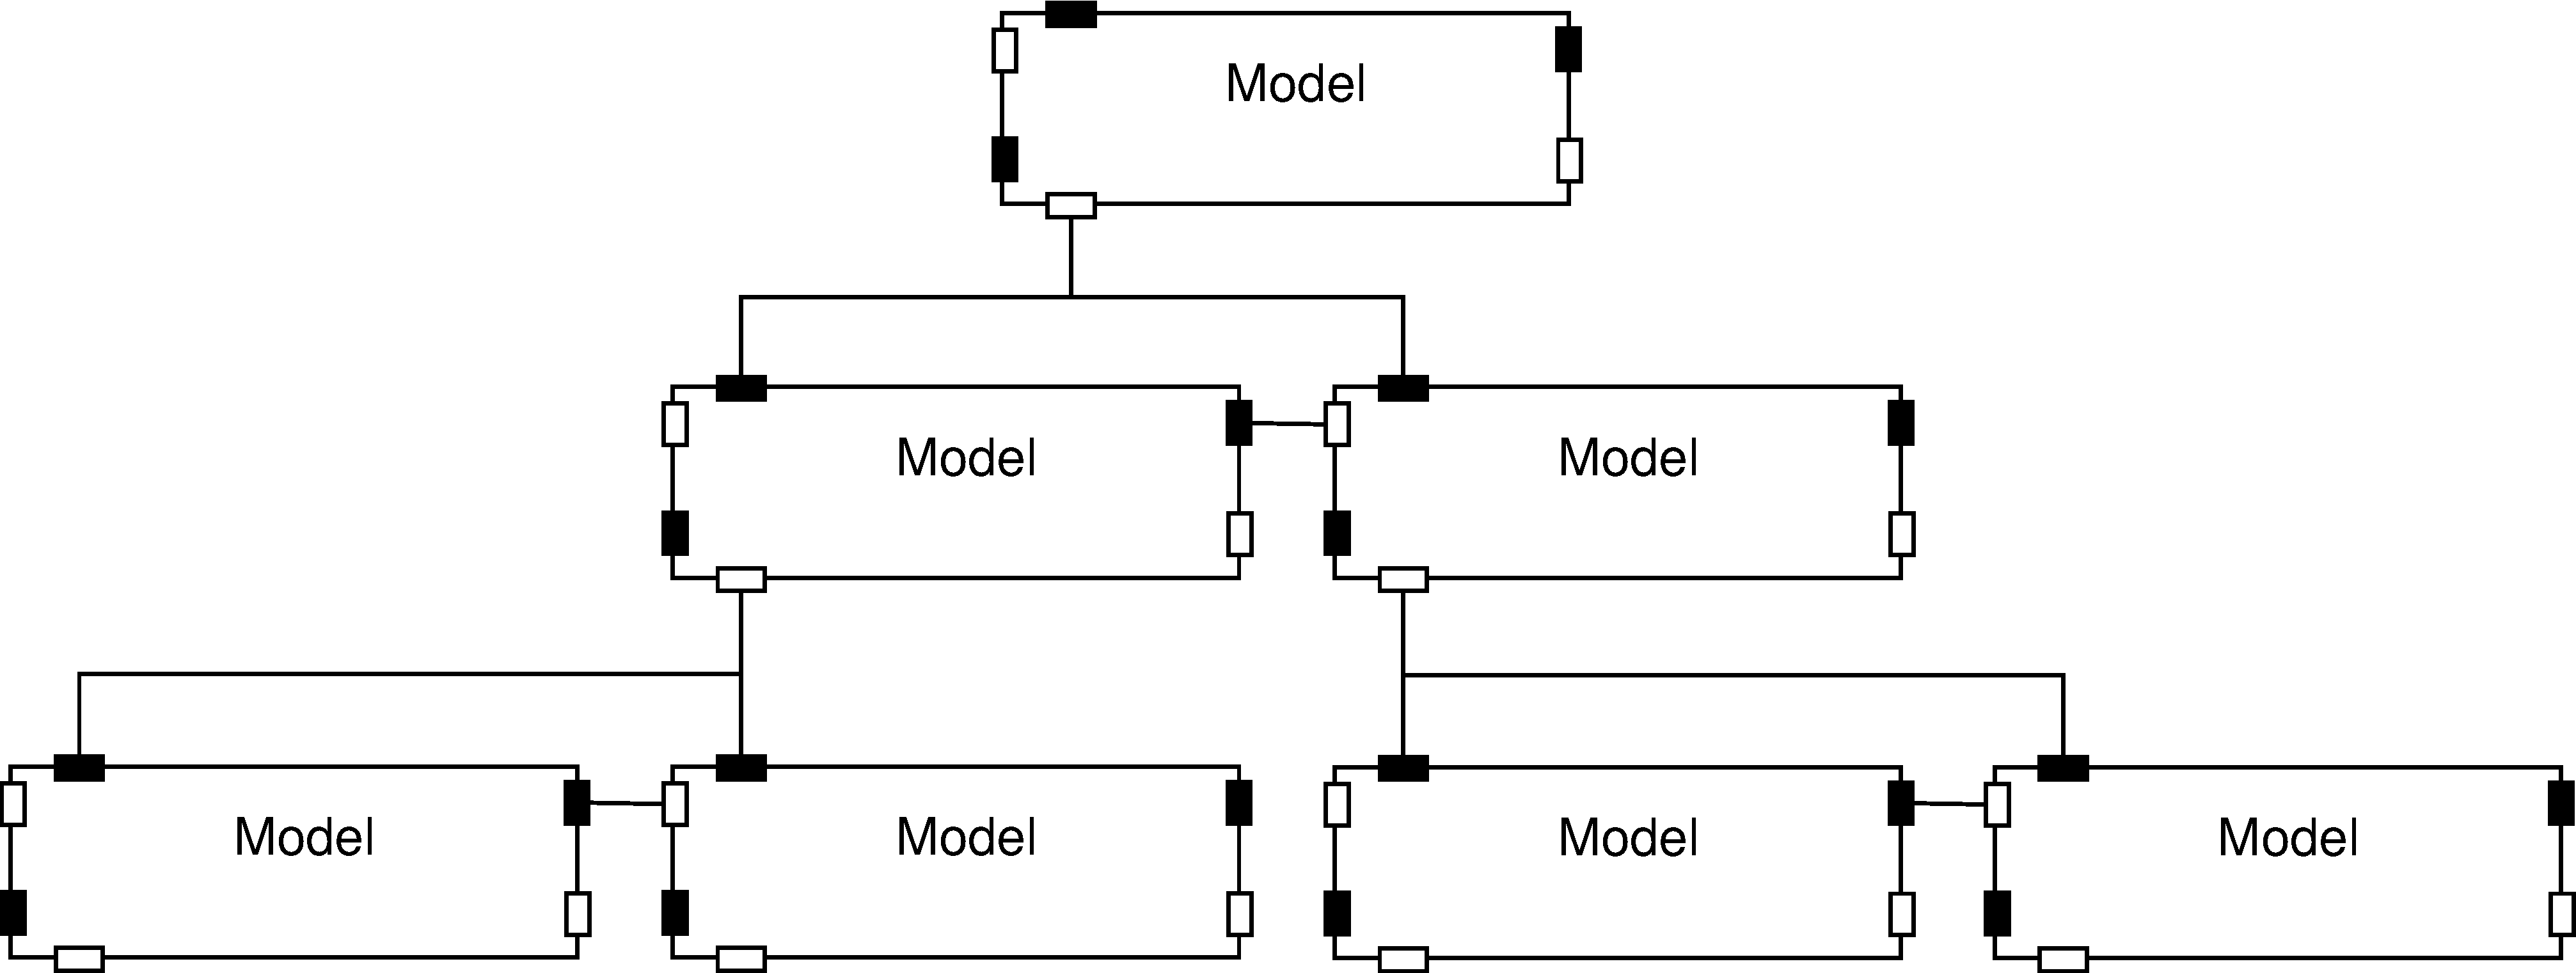
\includegraphics[width=\columnwidth]{fig/pholdtree.pdf}
    %TODO depth 1 but 3 levels deep?
    \caption{PHOLDTree model for depth 1 and width 2.}
    \label{fig:PHOLDTree_model}
\end{figure}

PHoldtree, like Queue, is a highly hierarchical model but one where the flattened structure cannot be partitioned into a chain as in Queue.
This topology is interesting since it highlights the effects of allocation.
This model allows us to investigate in depth the effects of non-cyclic allocation strategies and measure parallel speedup.
First, we evaluate the model in sequential simulation to provide a baseline for parallel simulation.

\subsubsection{Sequential Simulation}
Since adevs does not use direct connection, we expect a noticable performance difference between dxex and adevs.
This is shown in Figure~\ref{fig:PHOLDtree_seq_dn_benchmark}, where the fanout determines the performance penalty adevs suffers compared to dxex.
Profiling indeed indicated that an increase in width per subtree ($n$) leads to higher overheads in adevs due to the lack of direct connection.
Dxex uses direct connection, making it independent on fanout, but only of the number of models.
Slight deviations can still be seen, though, caused by the initialization overhead of direct connection.
Both adevs and dxex scale linearly in the number of atomic models.
We expect to see a similar distinction in parallel simulation.

\begin{figure}
    \center
    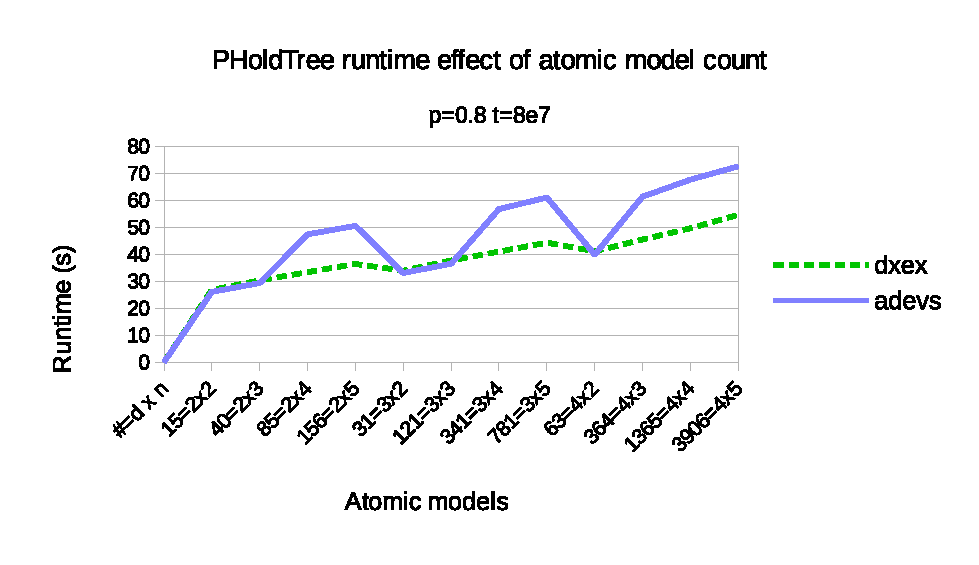
\includegraphics[width=\columnwidth]{fig/pholdtree_sequential_dn.eps}
    \caption{Effect of hierarchy in sequential simulation.}
    \label{fig:PHOLDtree_seq_dn_benchmark}
\end{figure}

\subsubsection{Parallel Simulation}
Next, we run the model using two different model allocation schemes: breadth-first and depth-first.
But first, we explain what we mean by both allocation schemes.

With breadth-first allocation, we traverse the tree in a breadth-first way, allocating subsequently visited atomic models to the same node.
This means, intuitively, that atomic models at the same level in the tree, but not necessarily siblings, are frequently allocated to the same node.
Since there is only infrequently some communication between siblings, and even never between different subtrees, this does not sound an intuitive allocation.
This allocation strategy is shown in Figure~\ref{fig:PholdTree_model_bfs}.

With depth-first allocation, we traverse the tree in a depth-first way, allocating subsequently visited atomic models to the same node.
This means, intuitively, that subtreees are frequently allocated to the same node.
This allocation strategy is shown in Figure~\ref{fig:PholdTree_model_dfs}.

The breadth first allocation scheme will result in kernels that will form a dependency chain with multiple branches, much like in the Queue model.
Such a linear dependency chain can result in a parallel speedup as we demonstrated with the Queue model, but this is not always true as we will demonstrate in this section.
A single kernel that has an unbalanced number of atomic models or unequal computation load in transition functions will slow down the remainder of the chain.
This effect is also apparent if the thread a kernel runs on is not fairly scheduled.
In conservative this will lead to excessive polling of the other kernels' EOT values, in optimistic this will lead to a cascade of reverts since dependent kernels will simulate ahead of the slower kernel.
In Figure~\ref{fig:pholdtree_visualize_parBFS} and Figure~\ref{fig:pholdtree_visualize_parDFS} the simulation trace is visualized for breadth-first and depth-first, respectively, highlighting the remarks made in this paragraph.

\begin{figure}
   \center
   
   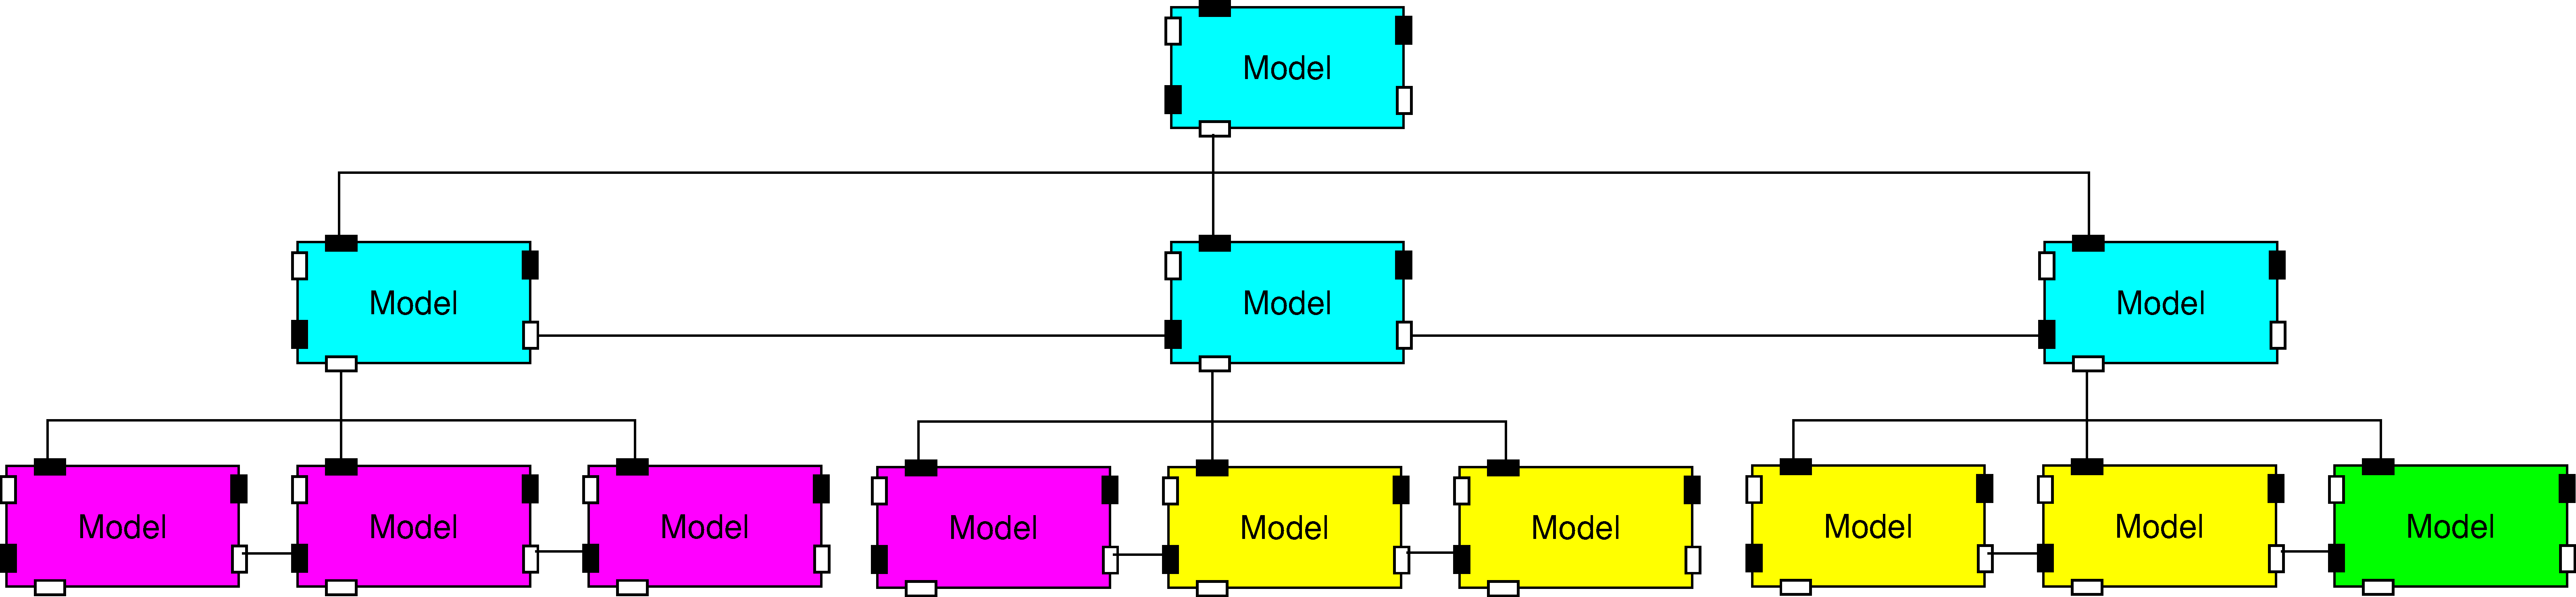
\includegraphics[width=\columnwidth]{fig/pholdtree_alloc_BF.pdf}
   \caption{PHOLDTree model breadth first allocation with 4 kernels.}
   \label{fig:PholdTree_model_bfs}
   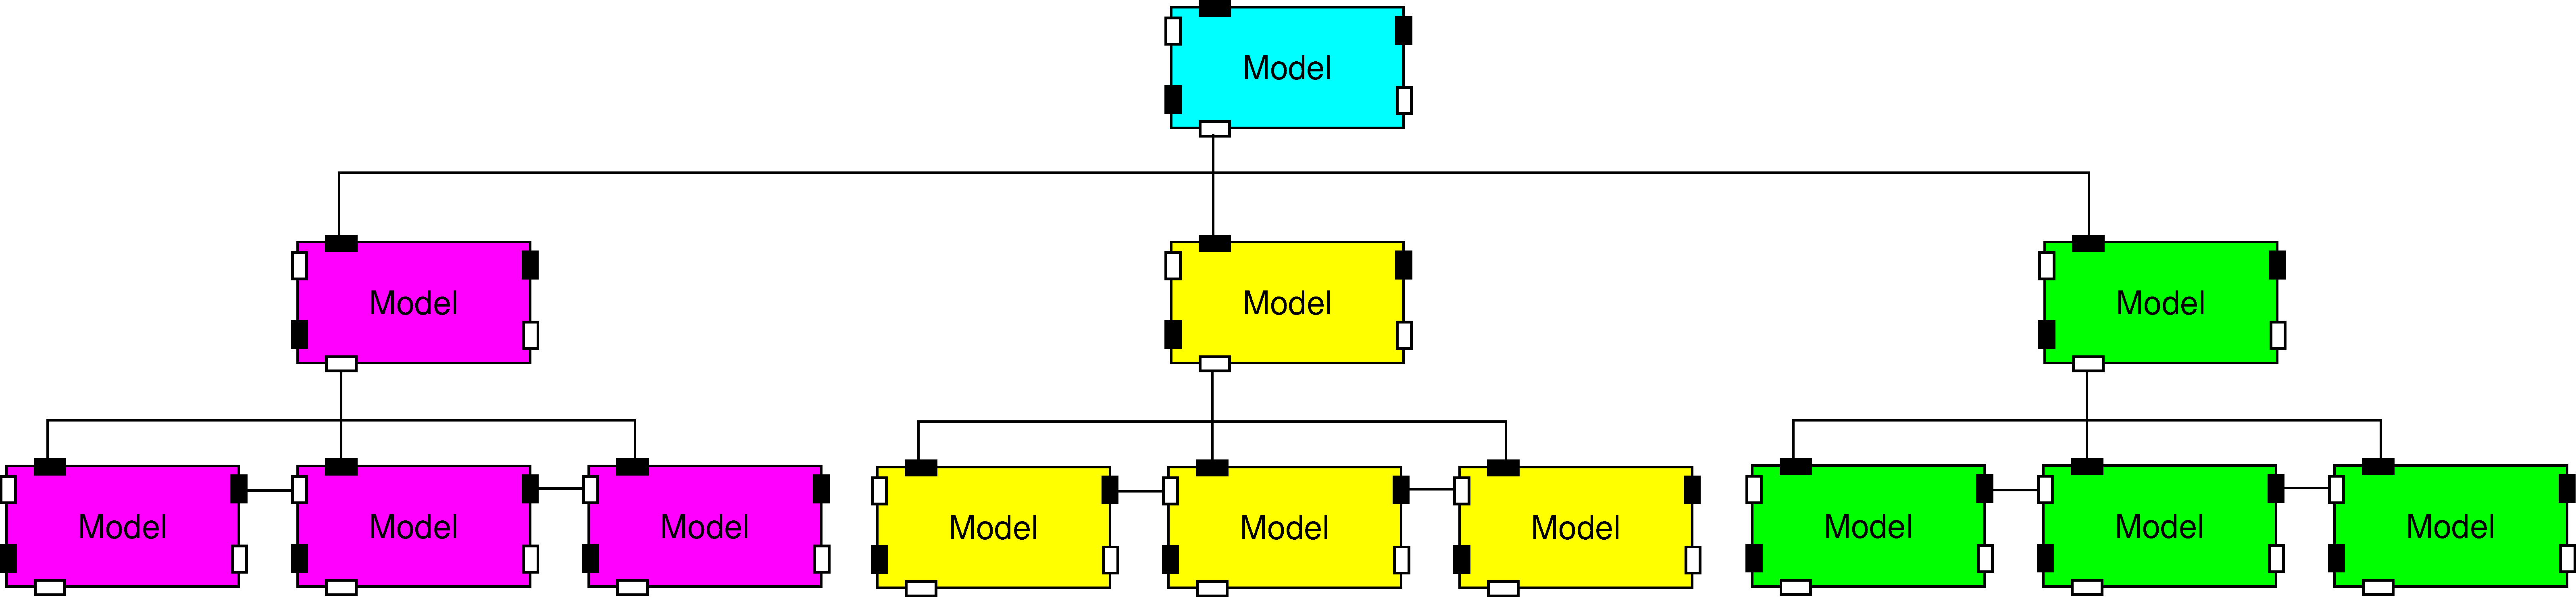
\includegraphics[width=\columnwidth]{fig/pholdtree_alloc_DF.pdf}
   \caption{PHOLDTree model depth first allocation with 4 kernels.}
   \label{fig:PholdTree_model_dfs}
\end{figure}

After simulation, the traces can be visualized for both breadth-first and depth-first allocation.
Using a breadth-first allocation scheme, as shown in Figure~\ref{fig:pholdtree_visualize_parBFS}, we notice that many events get exchanged between cores.
This is caused by the high number of inter-core connections and the high number of events exchanged over these connections.
The number of connections between nodes at the same simulation core is also rather low.
Using a depth-first allocation scheme, however, as shown in Figure~\ref{fig:pholdtree_visualize_parDFS},

\begin{figure}
    \center
    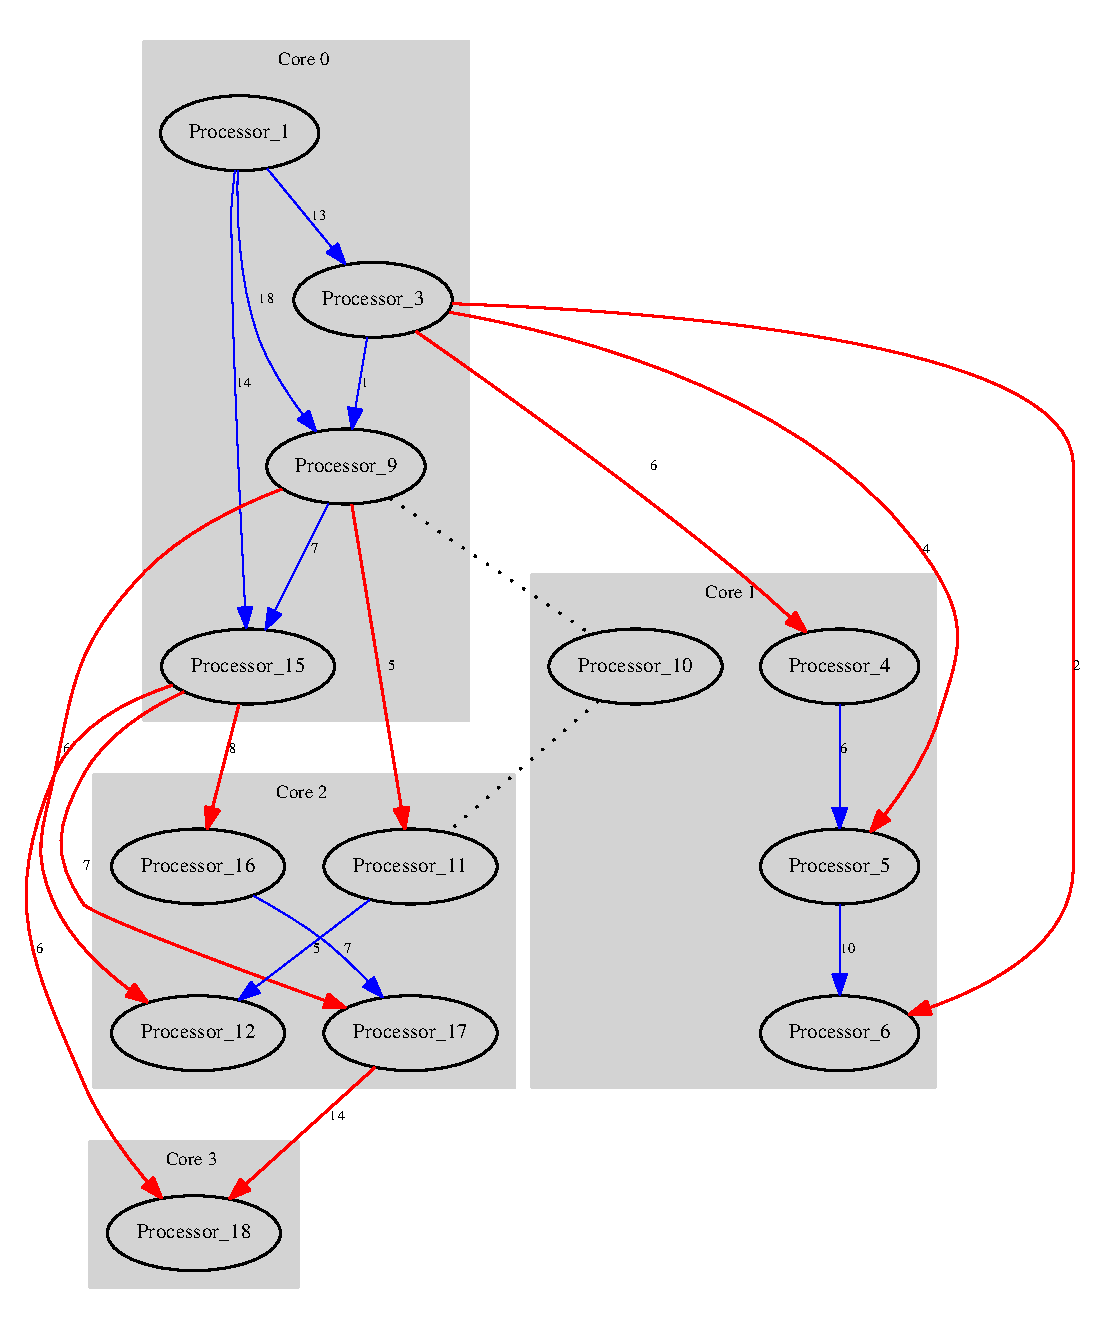
\includegraphics[width=\columnwidth]{fig/pholdtreed1n3t5000c4BFS.eps}
    \caption{Visualization of a PHOLDTree simulation with breadth first allocation and 4 kernels.}
    \label{fig:pholdtree_visualize_parBFS}
\end{figure}
\begin{figure}
    \center
    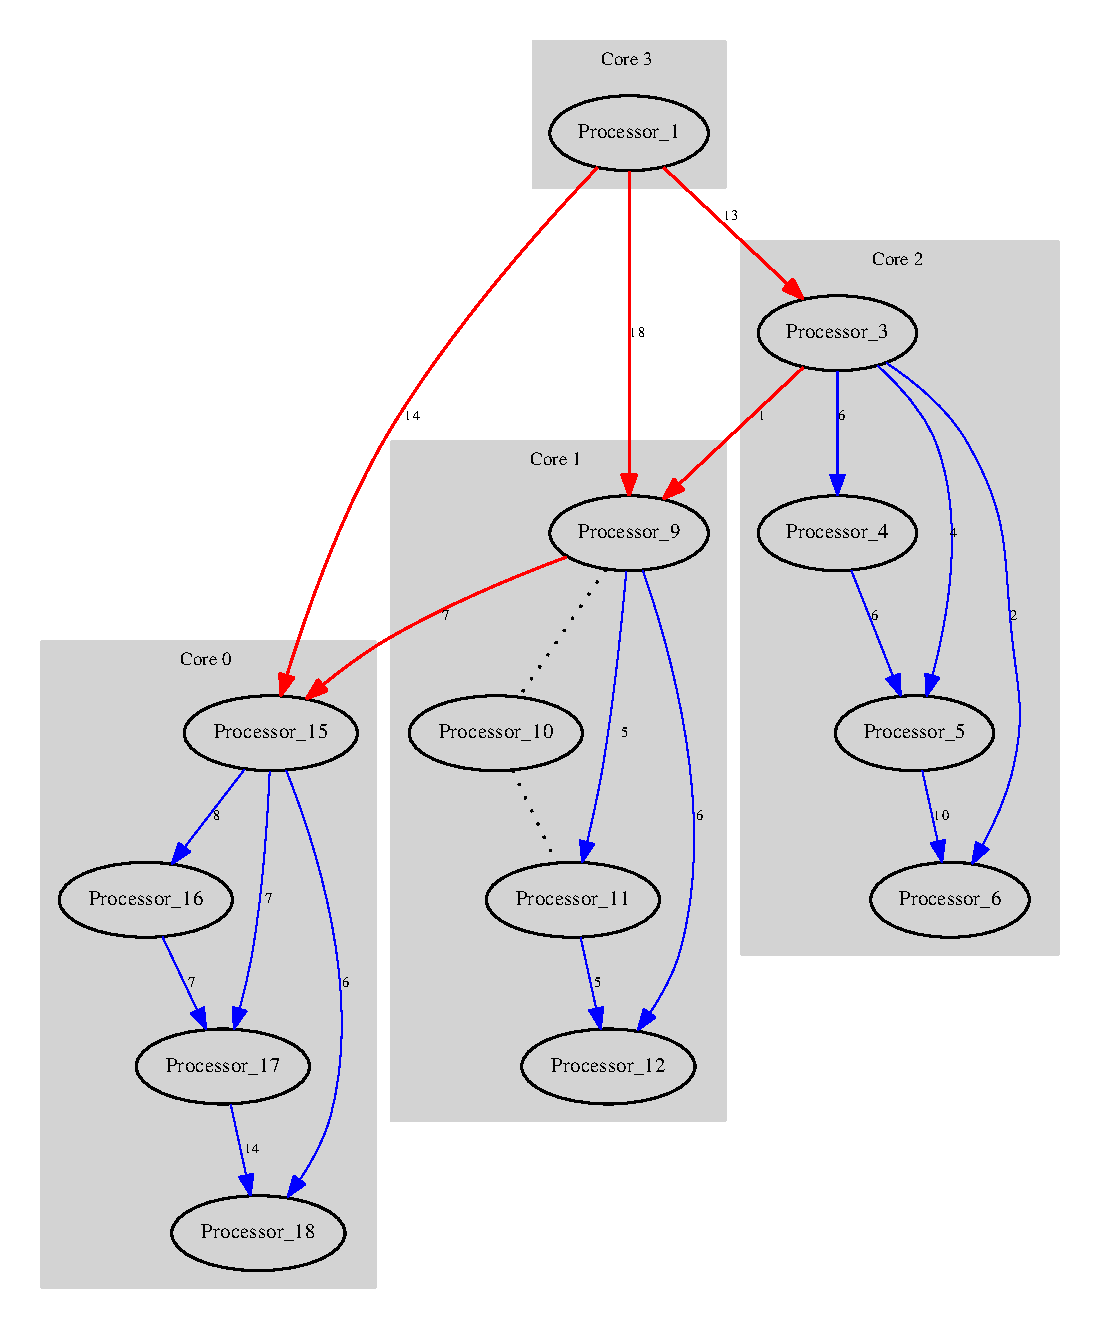
\includegraphics[width=\columnwidth]{fig/pholdtreed1n3t5000c4DFS.eps}
    \caption{Visualization of a PHOLDTree simulation with depth first allocation and 4 kernels.}
    \label{fig:pholdtree_visualize_parDFS}
\end{figure}

Simulation results are shown in Figure~\ref{fig:PholdTree_plot_alloc_high} for both allocation schemes in combination with both synchronization protocols.
We see that for both synchronization protocols, the depth-first allocation is significantly better than breadth-first allocation.
This is what we expected: depth-first allocation maintains locality better than breadth-first allocation.

The most prominent aspect of these results is the low performance for conservative depth-first allocation for two cores.
This is mostly caused by the difference between a sequential simulation and a parallel simulation: suddenly we need to take into account synchronization and passing around of lookahead values.
And since the number of cores is low, the overhead dominates any further speedup.
%TODO add some more explanation here maybe?
%TODO why is this not the case for optimistic?

%TODO this paragraph is strange: is this really the case?
Interestingly, we see that optimistic synchronization is less influenced by the allocation than conservative synchronization.
This is likely caused due to the lower number of connections to take into account in conservative synchronization.
Whereas conservative synchronization needs to take into account even scarcely used connections, optimistic synchronization does not.
The same is true in the opposite direction, though, where optimistic synchronization is slower when a good allocation is chosen.
Conservative synchronization will then be able to make better estimates, whereas optimistic synchronization does not make estimations.

\begin{figure}
    \center
    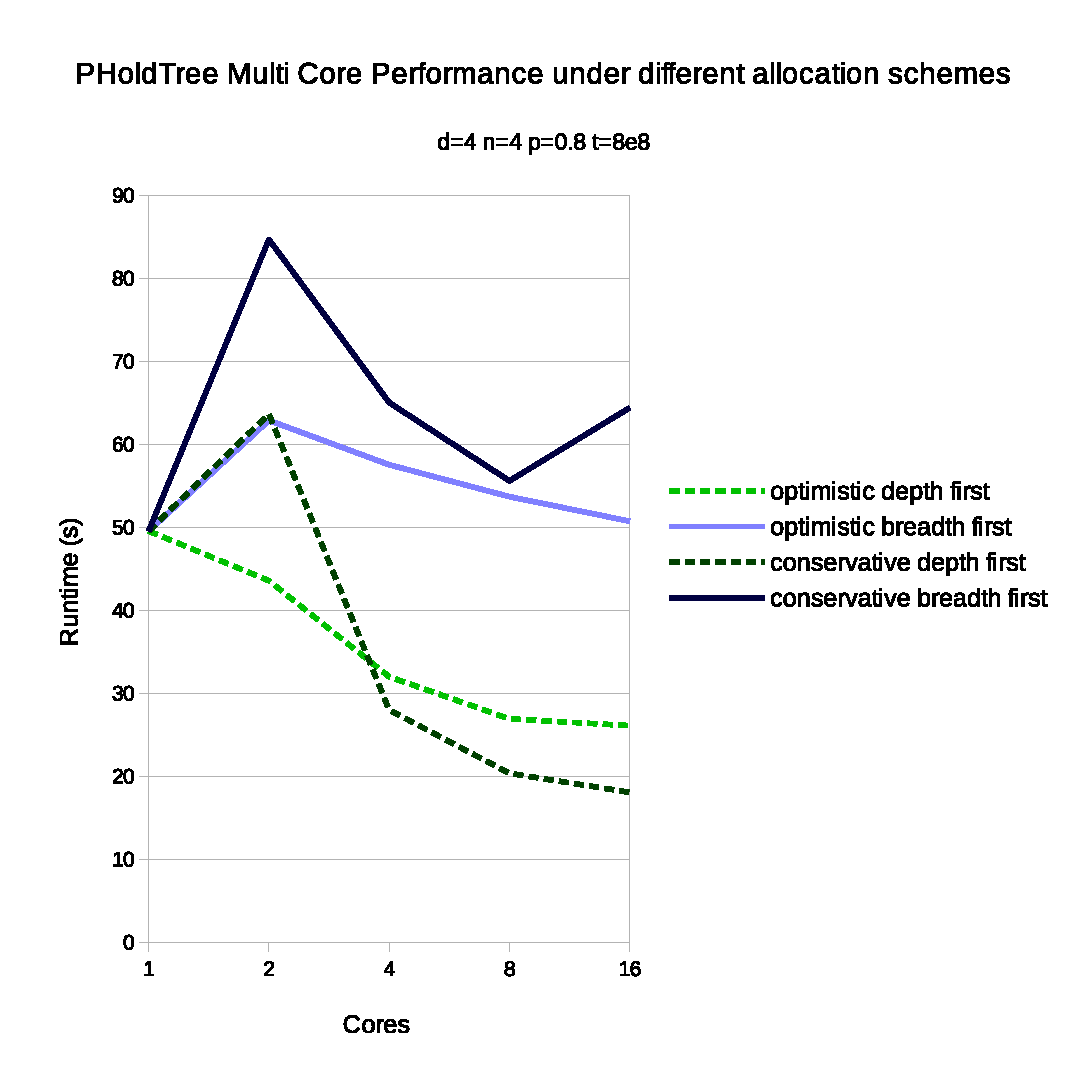
\includegraphics[width=\columnwidth]{fig/pholdtreeallochighp.eps}
    \caption{PHOLDTree model performance using different allocation schemes.}
    \label{fig:PholdTree_plot_alloc_high}
\end{figure}
